\chapter{Fundamentação}
\label{fundamentacao}


\section{Bases da Educação Profissional e Tecnológica}
\label{ept}

As instituições que compõem atualmente a Rede Federal de Educação Profissional, Científica e Tecnológica têm origem, em sua maioria, nas 19 escolas de aprendizes artífices criadas por decreto presidencial em 1909, durante o governo de Nilo Peçanha. \cite{silva2009institutos}. Originalmente subordinadas ao Ministério dos Negócios da Agricultura, Indústria e Comércio, essas escolas passaram, em 1930, a ser supervisionadas pelo recém-criado Ministério da Educação e Saúde Pública.


Em janeiro de 1937, a Lei nº 378 extinguiu as escolas de aprendizes artífices, substituindo-as pelos liceus industriais \cite{candido2019era}. Um ano após o ensino profissional ser considerado de nível médio, em 1942, os liceus passam a se chamar escolas industriais e técnicas, e, em 1959, escolas técnicas federais, configuradas como autarquias.

Ao longo desse mesmo tempo vai se constituindo uma rede de escolas agrícolas – Escolas Agrotécnicas Federais, com base no modelo escola fazenda e vinculadas ao Ministério da Agricultura \cite{silva2009institutos}. Em 1967, essas escolas fazendas passam para o então Ministério da Educação e Cultura tornando-se escolas agrícolas. Em 1978, três escolas federais, do Rio de Janeiro, Minas Gerais e Paraná são transformadas em Centros Federais de Educação Tecnológica (CEFET) equiparando-se, no âmbito da educação superior, aos centros universitários \cite{silva2009institutos}.

Em 29 de dezembro de 2008, a publicação da Lei 11.892, que no âmbito do Ministério da Educação criou os Institutos Federais de Educação, Ciência e Tecnologia, os quais apresentam um novo modelo de Educação Profissional, estruturados a partir dos CEFETs, escolas técnicas e agrotécnicas federais e escolas vinculadas às universidades federais \cite{garcia2018educaccao}.


Em 2019, já são mais de 661 unidades sendo estas vinculadas a 38 Institutos Federais, 02 Centros Federais de Educação Tecnológica (Cefet), a Universidade Tecnológica Federal do Paraná (UTFPR), a 22 escolas técnicas vinculadas às universidades federais e ao Colégio Pedro II \cite{conif2023}. 

Neste contexto, a Educação Profissional e Tecnológica (EPT) busca não apenas oferecer conhecimentos técnicos específicos, mas também desenvolver habilidades socioemocionais e competências transversais. A interdisciplinaridade torna-se essencial, permitindo aos estudantes uma formação mais abrangente e adaptável às constantes mudanças nas dinâmicas
profissionais. A EPT se sustenta em um tripé: Trabalho como princípio educativo; Politecnia e Formação humana integral, Figura \ref{fig:bases_ept}.

\begin{figure}[h!]
    \centering
    \caption{Bases Conceituais da EPT}
    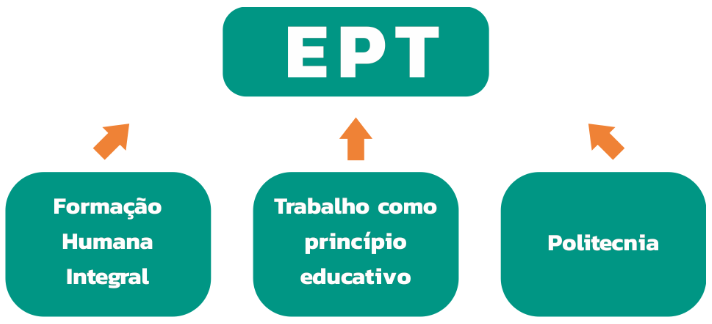
\includegraphics[scale=0.4]{figuras/bases_ept_v.png}
    \legend{Fonte: \citeonline{sousa2019guia}}
    \label{fig:bases_ept}
\end{figure}




\subsection{Trabalho Como Princípio Educativo}
\label{trab_prin_edu}

O trabalho é um processo central para a formação e a realização humanas, representando a interação com o mundo natural para a satisfação de necessidades básicas e complexas.

De acordo com \citeonline{frigotto2009teoria} , é por meio do trabalho que o ser humano transforma a natureza, atendendo tanto às suas necessidades básicas quanto às mais complexas, como culturais, lúdicas, estéticas e afetivas. \citeonline{de2018trabalho} destacam que o ser humano produz sua realidade e dela se apropria, motivo pelo qual o trabalho é um princípio educativo.


O trabalho como princípio educativo orienta a formação para a emancipação humana, para o desenvolvimento autônomo do ser rumo à expressão de suas potencialidades para transformação da realidade social coletiva. \citeonline{kulesza2019trabalho} registra que o trabalho como princípio educativo se relaciona com uma postura ativa e criativa perante o mundo.








\subsection{Politecnia}
\label{politecnia}

Derivado do trabalho como princípio educativo, o conceito de politecnia, segundo \citeonline{maciel2017fundamentos}, remonta às três dimensões da educação propostas por Karl Marx: educação intelectual, física e tecnológica - este último termo foi posteriormente modificado para educação politécnica.

O conceito de politecnia está relacionado à ideia de que a formação dos indivíduos deve abranger uma diversidade de conhecimentos e habilidades que vão além de uma única especialização técnica. Conforme apontado por autores como \citeonline{frigotto2005ensino}, a politecnia é uma resposta à fragmentação do trabalho e à alienação produzida pelo sistema capitalista, propondo a integração entre saberes científicos, técnicos, culturais e sociais.

Na prática, a politecnia se manifesta na organização curricular da EPT, que busca integrar disciplinas que tratam não apenas de técnicas específicas, mas também de áreas como ciências humanas, exatas e sociais aplicadas. Essa abordagem propõe que a formação profissional seja voltada para a compreensão das relações sociais e das dinâmicas produtivas como um todo, em vez de se limitar ao desenvolvimento de competências específicas para o mercado de trabalho \cite{ciavatta2005formaccao}.



\subsection{Formação Humana Integral}

% Formação humana integral ou ominilateral
A Formação Humana Integral também conhecida como \textbf{Formação Omnilatetal}, segundo \citeonline{saviani1994trabalho} concebe o trabalho como o ato de agir sobre a natureza, adaptando-a na base material indispensável para que seres humanos continuem existindo. O trabalho define a essência humana. Assim, o homem interage conscientemente com a natureza por ser seu meio direto de vida, fazendo-o pelo trabalho.

Em O Capital, \citeonline{marx1988capital} afirma que o trabalho é um processo entre o homem e a Natureza, "um processo em que o homem, por sua própria ação, media, regula e controla seu metabolismo com a Natureza". Os seres humanos são os artífices de sua própria história. Ao transformarem a natureza, os homens transformam a si próprios como seres humanos \cite{marx1984ideologia}. Assim corroboram \citeonline{frigotto2005trabalho}, que o trabalho como princípio educativo está vinculado à própria forma de ser dos seres humanos. O ser humano, para poder existir, vive de uma dependência com a natureza. E é pela ação vital do trabalho que ao transformarem a natureza, os homens também se transformam.




%\subsection{Institutos Federais de Educação, Ciência e Tecnologia}

%Uma das características centrais da formação da Rede Federal de Educação Profissional, Científica e Tecnológica (Rede Federal) foi a implantação de uma nova concepção sobre o papel e a presença do sistema de ensino federal na oferta pública da educação profissional e tecnológica \cite{mec2023}.

%Essa característica se materializa no desenho de um novo padrão de instituição, os denominados Institutos Federais de Educação, Ciência e Tecnologia (Institutos Federais ou IFs), estruturados a partir dos vários modelos existentes e da experiência e capacidade instaladas especialmente nos Centros Federais de Educação Tecnológica (Cefet), nas escolas técnicas e agrotécnicas federais e nas escolas técnicas vinculadas às universidades federais \cite{mec2023}.



%Os Institutos Federais são instituições, pluricurriculares e multicampi (reitoria, campus, campus avançado, polos de inovação e polos de educação a distância), especializados na oferta de educação profissional e tecnológica (EPT) em todos os seus níveis e formas de articulação com os demais níveis e modalidades da Educação Nacional, oferta os diferentes tipos de cursos de EPT, além de licenciaturas, bacharelados e pós-graduação stricto sensu.

%Instituídos no momento de constituição da Rede Federal, os institutos têm como obrigatoriedade legal garantir um mínimo de 50\% de suas vagas para a oferta de cursos técnicos de nível médio, prioritariamente na forma integrada.

%Devem, ainda, garantir o mínimo de 20\% de suas vagas para atender a oferta de cursos de licenciatura, bem como programas especiais de formação pedagógica, com vistas a formação de professores para a educação básica, sobretudo nas áreas de ciências e matemática, e para a educação profissional.

%\subsection{Universidade Tecnológica Federal do Paraná}

%A Universidade Tecnológica Federal do Paraná (UTFPR) é a primeira assim denominada no Brasil e, por isso, tem uma história um pouco diferente das outras universidades. A Instituição não foi criada e, sim, transformada a partir do Centro Federal de Educação Tecnológica do Paraná (Cefet-PR). Como a origem deste centro é a Escola de Aprendizes Artífices, fundada em 1909, a UTFPR herdou uma longa e expressiva trajetória na educação profissional \cite{utfpr2023}.

%A UTFPR tem como principal foco a graduação, a pós-graduação e a extensão. Oferece 100 cursos superiores de tecnologia, bacharelados (entre eles engenharias) e licenciaturas. Como também atende à necessidade de pessoas que desejam qualificação profissional de nível médio, a UTFPR oferta 19 cursos técnicos em diversas áreas do mercado, como técnicos de nível médio integrado  e cursos técnicos de nível médio subsequentes na modalidade a distância, com polos distribuídos pelos estados do Paraná e de São Paulo \cite{utfpr2023}. 

%A UTFPR configura-se como universidade especializada, pluridisciplinar, com foco na graduação e na pós-graduação, atuando ainda na área de pesquisa e extensão tecnológica. Foi instituída pela Lei nº 11.184/2005 a partir do Centro Federal de Educação Tecnológica do Paraná (Cefet-PR).

%\subsection{Centros Federais de Educação Tecnológica}

%Os Cefets são instituições de regime especial, de natureza pluricurricular e multiunidade (unidade sede e unidades de ensino descentralizada). Conforme estabelecido em sua lei de criação (Lei nº 6.545/1978), atuam na oferta de cursos de qualificação profissional, cursos técnicos de nível médio, cursos superiores de graduação – licenciatura, tecnologia e bacharelado –, de cursos superiores de pós-graduação lato e stricto sensu – especialização, mestrado e doutorado. A pesquisa aplicada e a extensão e desenvolvimento tecnológico também compõem sua missão \cite{mec2023}.

%Segundo o \cite{mec2023}, existem apenas dois Cefets: Centro Federal de Educação Tecnológica de Minas Gerais e Centro Federal de Educação Tecnológica Celso Suckow da Fonseca no Rio de Janeiro que compõem a rede de educação profissional e tecnológica assim como outras unidades (Escolas Técnicas e o Colégio Pedro II).



%\subsection{Escolas Técnicas Vinculadas}

%Instituições de ensino subordinadas à Secretaria de Educação Profissional e Tecnológica do Ministério da Educação (SETEC/MEC), dotadas de autonomia administrativa, didática e financeira – por tratarem-se de autarquias federais – e responsáveis por ofertar educação profissional, através de seus diversos cursos e programas, além do ensino médio \cite{paulo2023}. Constituem-se unidades de ensino pertencentes à estrutura organizacional das universidades federais.

%O Condetuf (Conselho Nacional de Dirigentes das  Escolas Técnicas Vinculadas às Universidades Federais) é a associação que congrega os dirigentes das Escolas Técnicas Vinculadas às Universidades Federais (ETVs) em todo território nacional, representando 23 instituições de ensino \cite{condetuf2023}.



%\subsection{Colégio Pedro II}

%Fundado em 2 de dezembro de 1837, o Colégio Pedro II é uma das mais tradicionais instituições públicas de ensino básico do Brasil. Ao longo de sua história, foi responsável pela formação de alunos que se destacaram por suas carreiras profissionais e influência na sociedade. Seu quadro de egressos possui presidentes da República, músicos, compositores, poetas, médicos, juristas, professores, historiadores, jornalistas, dentre outros \cite{cpii2023}.

%Em seus mais de 180 anos, o Colégio passou por períodos de expansão e modernização sem deixar de lado as características que o tornaram referência no cenário educacional brasileiro. Equiparado aos Institutos Federais de Educação, Ciência e Tecnologia, com a sanção da lei 12.677/12, o Colégio Pedro II conta com 14 campi, sendo 12 no município do Rio de Janeiro, um em Niterói e um em Duque de Caxias, e um Centro de Referência em Educação Infantil, localizado em Realengo \cite{cpii2023}.












%\section{Instituto Federal do Amapá}
%\label{ifap}

%A história do Instituto Federal do Amapá (IFAP) começa em 25 de outubro de 2007, com a criação da Escola Técnica Federal do Amapá (ETFAP), instituída pela Lei nº 11.534. Em 13 de novembro de 2007, a Portaria MEC nº 1066 atribui ao Centro Federal de Educação Tecnológica do Pará (CEFET/PA) o encargo de implantar a ETFAP. Para tomar a frente das articulações locais e viabilizar a implantação da então Escola Técnica Federal do Amapá, a Portaria MEC nº 1199, de 12 de Dezembro de 2007, nomeia o professor Emanuel Alves de Moura para exercer o cargo de Diretor-Geral Pró-Tempore \cite{ifap2022}.

%Em 29 de dezembro de 2008, a Lei nº 11.892, que institui a Rede Federal de Educação Profissional, Científica e Tecnológica, transforma a ETFAP em Instituto Federal de Educação, Ciência e Tecnologia do Amapá (Ifap) – autarquia vinculada ao Ministério da Educação, detentora de autonomia administrativa, patrimonial, financeira, didático-pedagógica e disciplinar, equiparada às universidades federais. Dando continuidade ao processo de implantação, o professor Emanuel Alves de Moura é nomeado reitor Pró-Tempore, pela Portaria MEC 021/2009, de 7 de janeiro de 2009 \cite{ifap2022}.

%Atualmente o IFAP possui 6 unidades, Câmpus Laranjal do Jari, Câmpus Macapá, Câmpus Agrícola Porto Grande, Câmpus Santana, Câmpus Avançado Oiapoque, Centro de Referência em EaD Pedra Branca, cada unidade com seus respectivos cursos de acordo com o arranjo produtivo local.







%\subsection{Unidade - Câmpus Macapá}
%\label{cmcp}

%O Câmpus Macapá inicia sua atividades de ensino no 2º semestre de 2010 com a oferta de 140 vagas para os cursos subsequentes de Técnico em Edificações, Técnicos em Mineração, Técnico em Alimentos e Técnico em Redes de Computadores. As primeiras turmas iniciaram na sede provisória Escola Estadual Darci Ribeiro, no bairro Novo Horizonte, cedida pelo Governo do Estado do Amapá (GEA) para o início das atividades administrativas de implantação do Instituto Federal Amapá \cite{ifapmacapa2022}.

%Em 2011, obedecendo ao processo de instalação e implementação, começaram a ser ofertados os demais cursos de Ensino Técnico de Nível Médio nas modalidades Integrado, Subsequente e Educação de Jovens e Adultos (PROEJA), cursos superiores de Licenciaturas e de Tecnologia, Pós-Graduação Lato Sensu e Stricto Sensu e Formação Inicial e Continuada – FIC. Nesse ano foram ofertados cursos FIC no âmbito dos programas federais: Programa Nacional de Acesso ao Ensino Técnico (PRONATEC) e o Programa Nacional Mulheres Mil (PNMM), bem como Profuncionário, voltado à capacitação do funcionalismo da rede pública estadual e municipal do Amapá. Naquele ano, devido o crescimento das atividades, a sede provisória do campus Macapá transfere-se para o Centro de Educação Profissional Graziela Reis de Souza, no centro da capital, cedida pelo Governo do Estado do Amapá \cite{ifapmacapa2022}.

%Em Fevereiro de 2012 as atividades administrativas e de ensino transferem-se para o prédio definitivo, localizado no bairro Brasil Novo, zona norte de Macapá, possibilitando a ampliação das atividades do IFAP na capital \cite{ifapmacapa2022}. O câmpus Avançado de Oiapoque está vinculado administrativamente ao campi Macapá.







\section{Tecnologias Digitais da Informação na Educação}
\label{tics_educacao}

A adoção de tecnologias para o ensino e a aprendizagem inclui os Recursos Educacionais Abertos (REA), surgidos em 2002 \cite{unesco2020}, como parte do conceito mais amplo de Educação Aberta (\textit{Open Education}), que, segundo \citeonline{inuzuka2012produccao}, "[...]  é um movimento de pessoas e instituições que promovem ações com o objetivo tornar a educação mais livre e acessível para todos".

Para os autores \citeonline{niskier1993tecnologia} e \citeonline{da2021educaccao}, vem de longa data ressaltando o papel da tecnologia na educação, destacando sua evolução ao longo do tempo. Desde o ábaco, utilizado por povos primitivos, até os modernos computadores, a tecnologia tem moldado a forma como aprendemos e ensinamos, promovendo assim a integração de forma bidirecional de forma a facilitar adoção e engajamento.

Neste contexto, as mudanças nas práticas educacionais com o uso de mais recursos tecnológicos digitais e ou analógicos como instrumento ao educador de forma a facilitar o processo e a melhoria da aprendizagem. Na perspectiva dos autores \citeonline{maciel2012objetos}, "O uso de materiais didático-tecnológicos [...] à disposição do professor para reutilização em diversos contextos, dá mostra de que a parceria entre conteúdo, tecnologia e metodologia é bem-sucedida e, se incentivada, a tendência e aumentar o ganho no processo educacional".


Segundo \citeonline{xavier2013educaccao}, a adoção das Tecnologias Digitais de Informação e Comunicação (TDIC) na educação já não é mais uma questão a ser debatida, mas sim como utilizá-las de forma eficaz. Discute-se agora como utilizá-las para auxiliar o docente a trabalhar a diversidade de conteúdos presentes nas disciplinas do currículo escolar na forma de disciplinaridade, interdisciplinaridade, multidisciplinaridade e transdisciplinaridade de forma alternada.

Existe uma certa resistência para com os profissionais docentes para a mudança de paradigma principalmente quanto a aplicação de novas tecnologias, o autor \citeonline{fava2018trabalho} remete a critica. Essa resistência leva a uma serie de fatores que acarretam no "ossificação" da prática docente em detrimento da necessidade de utilizar novas TDIC.

Os currículos atuais, em sua maioria, são construídos por especialistas com opiniões tendenciosas, previsíveis, almas ideológicas, pois desejam a manutenção dos padrões tradicionais e a preservação dos benefícios adquiridos. Em outros cenários, são leais às suas teses de estudos, tendo dificuldades de descartar partes de todo o tecido do conhecimento de seu campo, mesmo que estes já se encontrem desatualizados \cite{fava2018trabalho}.

Na perspectiva de \citeonline{oliveira1997vygotsky}, explica que os sistemas simbólicos são estruturas complexas e articuladas que serão organizadas por meio de signos e instrumentos que são os chamados elementos mediadores. Na Figura \ref{fig:elementos_mediadores} mostra a relação e associa a ação do homem como meio ou mediador do processo de ensino-aprendizagem.

\begin{figure}[h!]
    \caption{Elementos Mediadores}
    \centering
    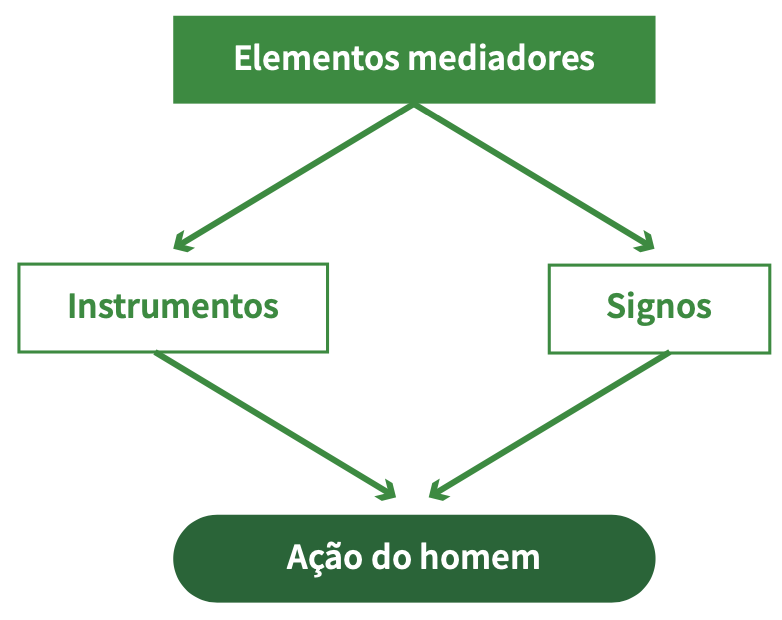
\includegraphics[scale=0.6]{figuras/elementos_mediadores.png}
    \label{fig:elementos_mediadores}
    \legend{Fonte: \citeonline{camillo2018teorias}}
\end{figure}

A mediação, segundo Vygotsky, é o processo pelo qual a ação do sujeito sobre o objeto é mediada por um determinado elemento. Por exemplo, a ação de um pintor sobre sua obra é mediada pelo pincel. Neste exemplo o elemento mediador (pincel) possibilita a transformação do objeto (quadro). Esta etapa intermediária “pincel -> quadro” é denominada mediação. Então, mediação é o processo de intervenção de um elemento intermediário numa relação - a relação deixa de ser direta e passa a ser mediada por esse elemento \cite{richit2004implicaccoes}.


Para Vygotsky as pessoas não tem um contato direto com objetos e sim uma mediação, por meio de um conhecimento ou por uma experiência, logo, ele defende a sua teoria como \textbf{sócio construtivista}, em que a interação é mediada por várias relações, vindo a se diferenciar do construtivismo, em que o indivíduo age sem desvios indo direto ao objetivo \cite{magalhaes2007perspectiva}.






Nesse sentido, \citeonline{ponte1988computador} acredita que os professores não devem deixar se reduzir ao papel de “correias de transmissão” de forma a utilizar em seu ensino produtos educacionais padronizados e prontos para usar.


Conforme citado por \citeonline{litto2009educaccao}, os novos modelos de aprendizagem utilizam intensamente as TIC e coincidem com a inovação em todos os níveis da vida humana. As novas tecnologias inserem-se no meio em que vivemos atualmente, o que impulsiona um conhecimento cada vez mais amplo, e por isso devemos utilizá-las como instrumento auxiliar no processo de ensino-aprendizagem. Nesse sentido \cite{richit2004implicaccoes}:

\begin{citacao}
Nesta perspectiva, a interferência da escola faz-se necessária no sentido de oferecer ao aluno oportunidades significativas de construção de conhecimentos e valores que estão atrelados à atual conjuntura social e, principalmente, promovendo a utilização das tecnologias informáticas como instrumentos auxiliares à prática pedagógica com o objetivo de promover interação, cooperação, comunicação e motivação a fim de diversificar e potencializar as relações inter e intrapessoais mediante situações mediatizadas, que venham a dar um novo significado ao processo de aprendizagem. Isto é, as relações entre sujeitos e, entre sujeitos e tecnologias colabora para a estruturação do conhecimento do grupo que a utiliza, bem como para o desenvolvimento desses sujeitos, o que caracteriza o coletivo seres humanos com mídias, proposto por \citeonline{levy1993tecnologias}.
\end{citacao}

De acordo com \citeonline{pais2002tecnologias} as tecnologias digitais ou software devem ser ajustados à linguagem dos alunos, isto é, devem apresentar uma interface de fácil interação, determinando a necessidade de serem avaliados segundo padrões vistos não somente sob o ponto de vista do nível de cognição e do valor do \textit{feedback}, mas segundo padrões culturais do sujeito.

Portanto, se as tecnologias informáticas fazem parte do contexto do aluno, então, a interação entre ambos (indivíduo/computador) precisa ser investigada como forma de favorecer o aprendizado e contribuir à construção do conhecimento \cite{richit2004implicaccoes}.





\section{Base Nacional Comum Curricular e a Matemática}
\label{bncc_mat}

A Base Nacional Comum Curricular (BNCC) é um documento normativo que estabelece as aprendizagens essenciais e progressivas que todos os estudantes devem adquirir ao longo das etapas e modalidades da Educação Básica \cite{bncc}.


Conforme definido na Lei de Diretrizes e Bases da Educação Nacional (LDB, Lei nº 9.394/1996), a Base deve nortear os currículos dos sistemas e redes de ensino das Unidades Federativas, como também as propostas pedagógicas de todas as escolas públicas e privadas de Educação Infantil, Ensino Fundamental e Ensino Médio, em todo o Brasil \cite{bncc}.

A Base estabelece conhecimentos, competências e habilidades que se espera que todos os estudantes desenvolvam ao longo da escolaridade básica. Orientada pelos princípios éticos, políticos e estéticos traçados pelas Diretrizes Curriculares Nacionais da Educação Básica, a Base soma-se aos propósitos que direcionam a educação brasileira para a formação humana integral e para a construção de uma sociedade justa, democrática e inclusiva \cite{bncc}.





%\section{Metodologias Ativas e Inovadoras na Educação}
%\label{metodologias_ativas}


%Diante árdua tarefa de dinamizar a prática docente, \citeonline{hartwig2019metodologias} afirmam que as metodologias ativas, em especial o ensino híbrido, com a ajuda dessas ferramentas síncronas e assíncronas, está sendo inserida nos sistemas educacionais, buscando inovar e ampliar a criatividade e a motivação.

%Conforme \citeonline{bacich2015aprender}, versar acerca de metodologias ativas implica partir do pressuposto de que não há um único modo de ensinar e de aprender. \citeonline{moran2015mudando} recomenda que as metodologias ativas sejam: “[...] pontos de partida para avançar para processos mais avançados de reflexão, de integração cognitiva, de generalização, de reelaboração de novas práticas”.

%Para \citeonline{barbosa2013metodologias} reforçam que, se a prática de ensino favorecer no estudante as ações de ouvir, ver, perguntar, discutir, fazer e ensinar, estar-se-á no caminho da aprendizagem ativa. De acordo com \citeonline{inocente2018metodologias}, utilizar metodologias ativas conduz a formação crítica de futuros profissionais, proporcionando o desenvolvimento de estudantes autônomos, criativos, críticos, interessados e firmes na tomada de decisões.



%\subsection{Gamificação no Ensino}
%\label{gamificicao}
%Do inglês “gamification”, a expressão gamificação foi assim intitulada pelo autor \cite{pelling2011short} adquiriu notabilidade por volta de 2010 apesar de ter surgido nos anos iniciais de 2000. Esta, como uma estratégia inovadora para o ambiente educacional, visa permitir uma vasta utilização de elementos e técnicas identificados e demasiadamente utilizados nos jogos no intuito de prover um cenário desafiador, obedecendo aos seguintes objetivos, mencionados por \cite{borges2013}, a saber:

%\begin{citacao}
%(1) aprimorar determinadas habilidades; (2) propor desafios que dão propósito/contexto a aprendizagem; (3)
%engajar os alunos em atividades mais participativas, interativas e interessantes; (4) maximizar o aprendizado de um determinado conteúdo; (5) promover a mudança de comportamento premiando ações adequadas e penalizando as inadequadas; (6) oferecer mecanismos de socialização e aprendizagem em grupo; e, finalmente, (7) discutir os benefícios da gamificação na motivação dos alunos para propor soluções aos diversos problemas de aprendizagem.
%\end{citacao}


%Um dos principais objetivos da gamificação é despertar o interesse dos estudantes para o processo de ensino e aprendizagem \cite{fardo2013gamificaccao}. Para \citeonline{sales2017gamificaccao}, gamificar a sala de aula não significa necessariamente criar um game, ou colocar a turma para jogar na sala de aula, mas consiste em usar as mesmas estratégias, métodos e pensamentos e alguns elementos do design de games no ambiente de aprendizagem, a saber: interação, colaboração, feedback, fases, desafios, motivação, regras claras dentre outros. 





















